\documentclass[12pt,a4paper]{article}
\usepackage[utf8]{inputenc}
\usepackage[german]{babel}
\usepackage{amsmath}
\usepackage{amsfonts}
\usepackage{amssymb}
\usepackage{graphicx}
\usepackage{tikz}
\usepackage{url}
\usepackage[left=2cm,right=2cm,top=2cm,bottom=2cm]{geometry}

\begin{document}
\parskip1.5em
\parindent0ex

\begin{titlepage}
\title{Multicoptersteuerung\\
\small{CCS Projektarbeit: Planung und Kalkulation}}
\author{Michael Wörner \and Christian Silfang}
\date{\today}
\end{titlepage}

\maketitle

\section{Komponenten für Quadrocopter}

\subsection*{Motoren und Rotoren}

Für den Quadrocopter werden vier Motoren und dazu passende Propeller benötigt. Die farblichen Unterschiede zeigen zusammengehörige Propeller-Paare. Davon werden jeweils 2 Stück linksdrehend und zwei Stück rechtsdrehend benötigt. Die Flugrichtung ist durch den blauen Pfeil dargestellt.
\vspace{1cm}
\begin{center}
\begin{tikzpicture}
% erste konfiguration
\node[color=black, fill=orange, opacity=0.8, circle, inner sep=0.4cm] (A) at (0,0) {3};
\node[color=gray, draw, opacity=0.8, circle, inner sep=0.2cm, loosely dashed] (AA) at (0,0) {};
\node[color=gray, draw, opacity=0.8, circle, inner sep=0.3cm, loosely dashed] (AAA) at (0,0) {};

\node[color=black, fill=green, opacity=0.8, circle, inner sep=0.4cm] (B) at (2,0) {4};
\node[color=gray, draw, opacity=0.8, circle, inner sep=0.2cm, loosely dashed] (BB) at (2,0) {};
\node[color=gray, draw, opacity=0.8, circle, inner sep=0.3cm, loosely dashed] (BBB) at (2,0) {};

\node[color=black, fill=green, opacity=0.8, circle, inner sep=0.4cm] (C) at (0,2) {1};
\node[color=gray, draw, opacity=0.8, circle, inner sep=0.2cm, loosely dashed] (CC) at (0,2) {};
\node[color=gray, draw, opacity=0.8, circle, inner sep=0.3cm, loosely dashed] (CCC) at (0,2) {};

\node[color=black, fill=orange, opacity=0.8, circle, inner sep=0.4cm] (D) at (2,2) {2};
\node[color=gray, draw, opacity=0.8, circle, inner sep=0.2cm, loosely dashed] (DD) at (2,2) {};
\node[color=gray, draw, opacity=0.8, circle, inner sep=0.3cm, loosely dashed] (DDD) at (2,2) {};

\draw[black, very thick] (A) -- (D);
\draw[black, very thick] (B) -- (C);

\draw[blue, very thick, ->] (1,1.8) -- (1,3);

\end{tikzpicture}
\end{center}

\subsubsection*{Motor: Suppo A2208/17 1100KV Brushless Outrunner}
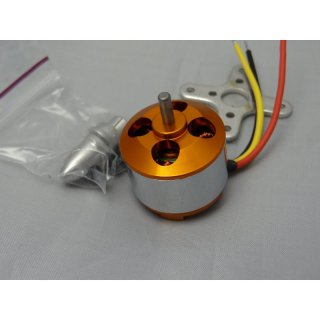
\includegraphics[scale=0.4]{Bilder/Suppo22082212.jpg}

\textbf{Preis:} 13,95 Euro

\subsubsection*{Motor: Suppo A2212/13 1000KV Brushless Outrunner}
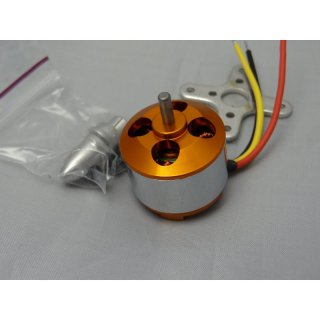
\includegraphics[scale=0.4]{Bilder/Suppo22082212.jpg}

\textbf{Preis:} 14,95 Euro

\subsubsection*{Motor: T-Motor MT1306 3100KV 2.0}
Motoren für einen Nanoquad.\footnote{\url{http://flyduino.net/Nanoquad-Rahmen}}

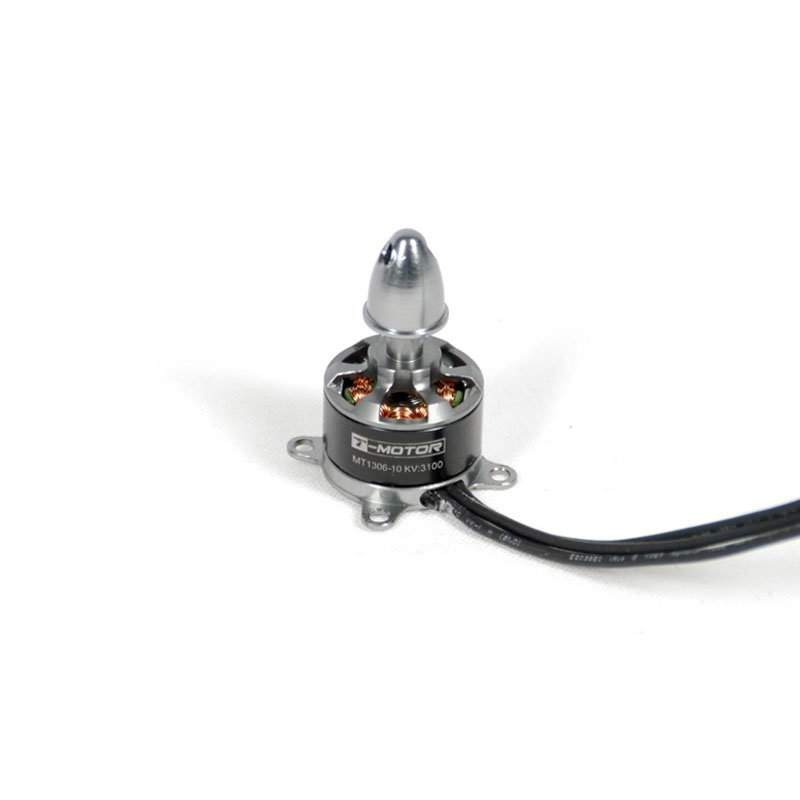
\includegraphics[scale=0.2]{Bilder/T-Motor.jpg}

\textbf{Preis:} 29,90 Euro

\subsubsection*{Propeller: 8"x4.5 Propeller Set 2 CW and 2 CCW}
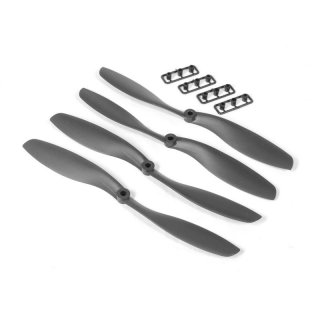
\includegraphics[scale=0.5]{Bilder/8Propeller.jpg}

\textbf{Preis:} 4,20 Euro

\subsubsection*{Propeller: 5030 Propeller Set 4 CW and 4 CCW}
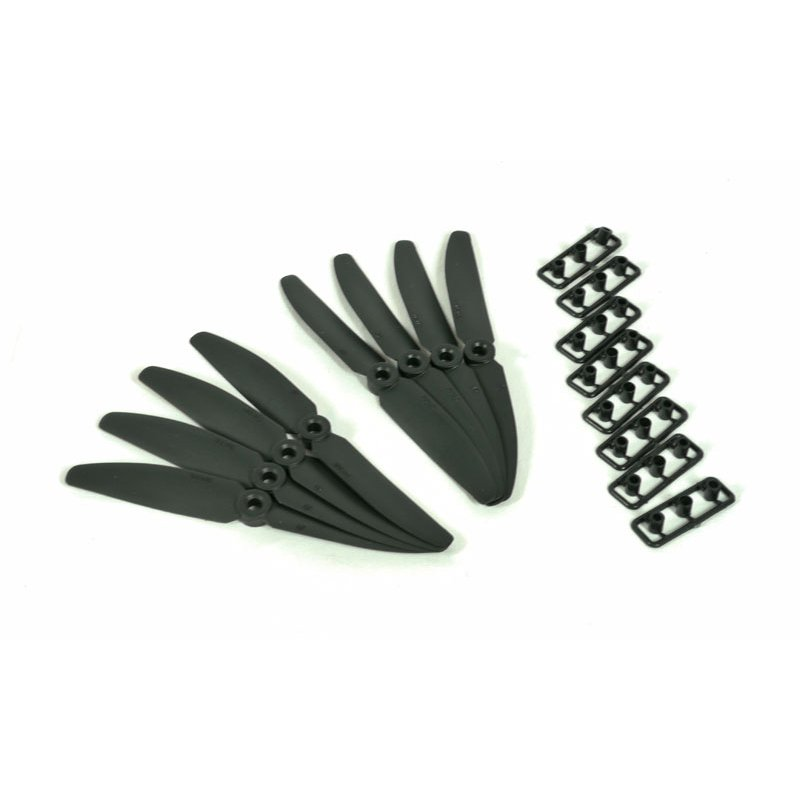
\includegraphics[scale=0.3]{Bilder/5Propeller.jpg}

\textbf{Preis:} 6,50 Euro

\subsection*{Motorsteuerungen (ESCs)}
ESCs sind verantwortlich für die Steuerung der einzelnen Motoren. Sie regeln, wie schnell sich ein Motor und damit der Propeller, dreht. Jeder Motor benötigt einen eigenen ESC.

\subsubsection*{Flyduino 10A ESC SimonK Firmware}
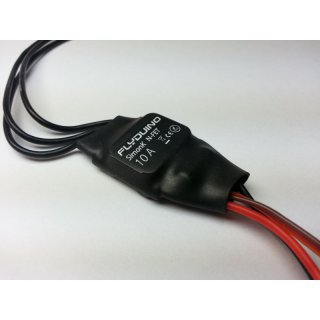
\includegraphics[scale=0.5]{Bilder/ESC10A.jpg}

\textbf{Preis:} 15,90 Euro

\subsubsection*{Flyduino NFET (HEXFET) 20A ESC SimonK Firmware}
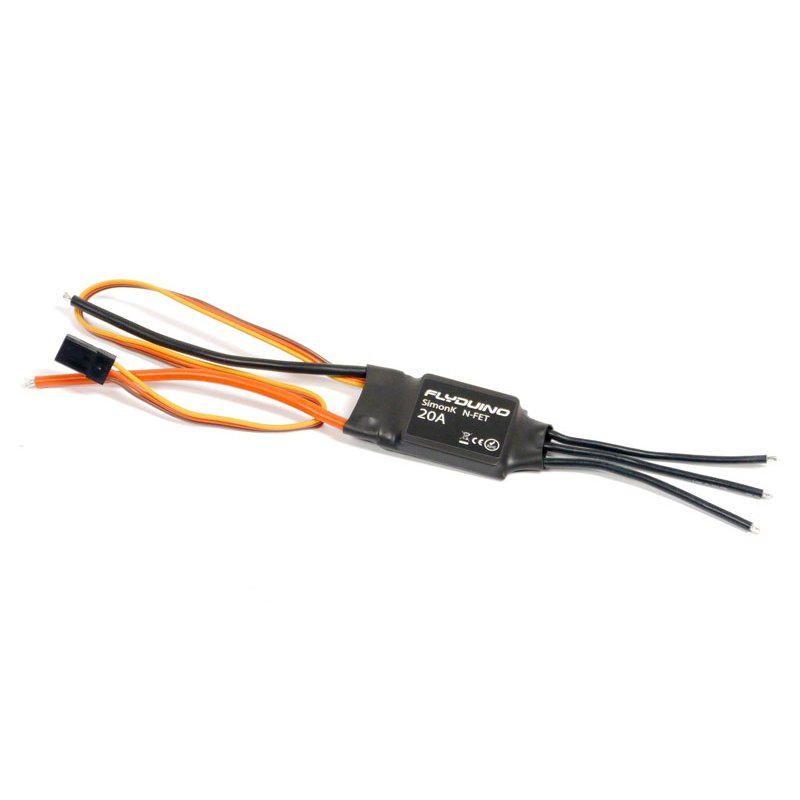
\includegraphics[scale=0.3]{Bilder/ESC20A.jpg}

\textbf{Preis:} 16,99 Euro

\subsubsection*{Flyduino 7A - BLHELI ESC}
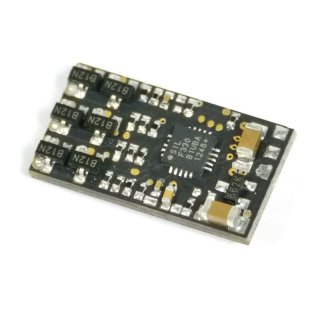
\includegraphics[scale=0.4]{Bilder/ESC7A.jpg}

\textbf{Preis:} 12,49 Euro

\subsection*{Flugcontroller}

\subsubsection*{NanoWii - ATmega32u4 Based MultiWii FC}
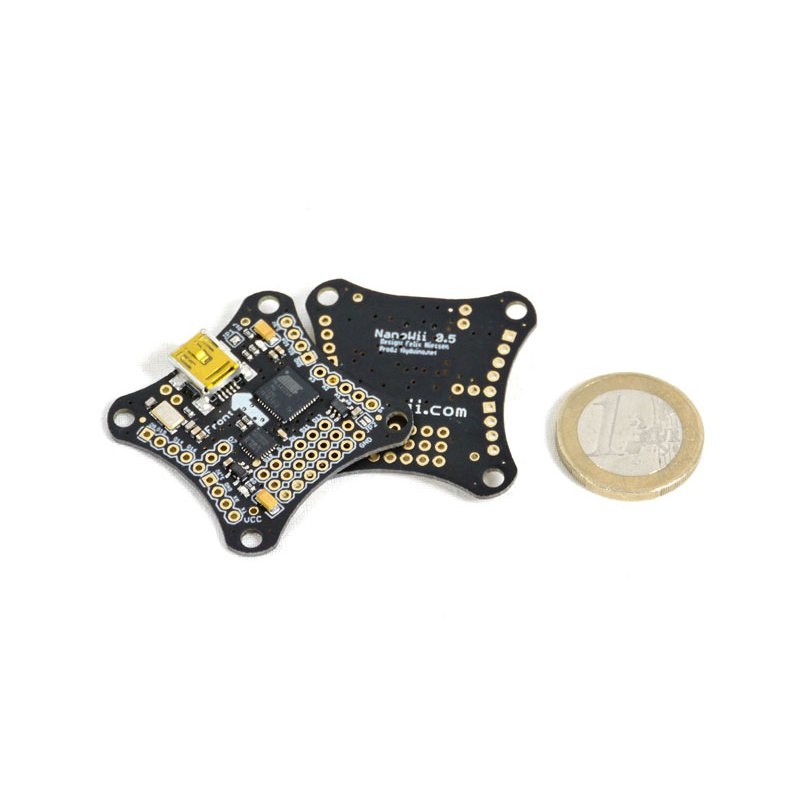
\includegraphics[scale=0.4]{Bilder/NanoWii.jpg}

\textbf{Preis:} 38,90 Euro

\subsubsection*{CRIUS ALL IN ONE PRO v1.0 Multi Rotor Flight Controller}
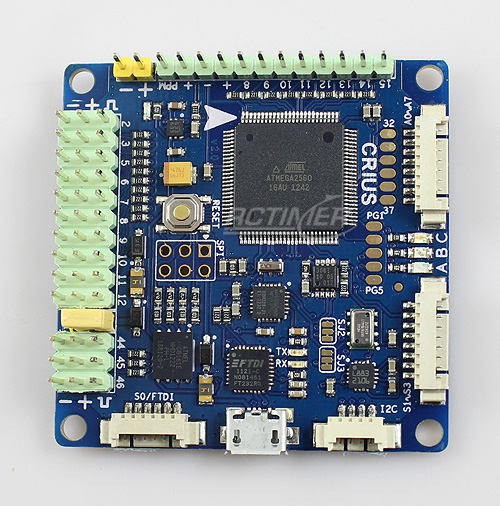
\includegraphics[scale=0.3]{Bilder/crius.jpg}

\textbf{Preis:} 58,26 USD

\subsubsection*{Flyduino MW32 v2 with 2.3 preloaded}
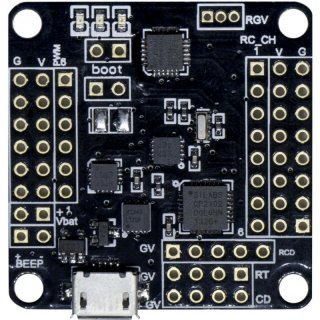
\includegraphics[scale=0.4]{Bilder/MultikopterFC2.jpg}

\textbf{Preis:} 47,90 Euro

\subsection*{Rahmen und Ausleger}
Variabel in der Größe. Nanoquad bspw. 17cm x 17cm groß. Herkömmlicher Quadrocopter hat Aluausleger von 20cm. Abzüglich eines Rahmens eine Komplettabmessung von ca. 32cm x 32cm. 

\subsubsection*{Nanoquad Rahmen}
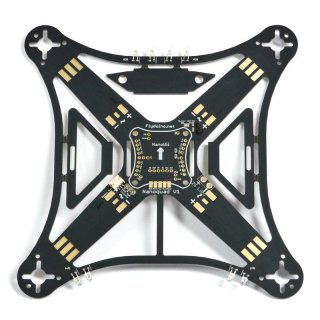
\includegraphics[scale=0.5]{Bilder/Nanoquad-Rahmen.jpg}

\textbf{Preis:} 34,99 Euro

\subsubsection*{Quadrokopter Rahmen Set 20cm arm}
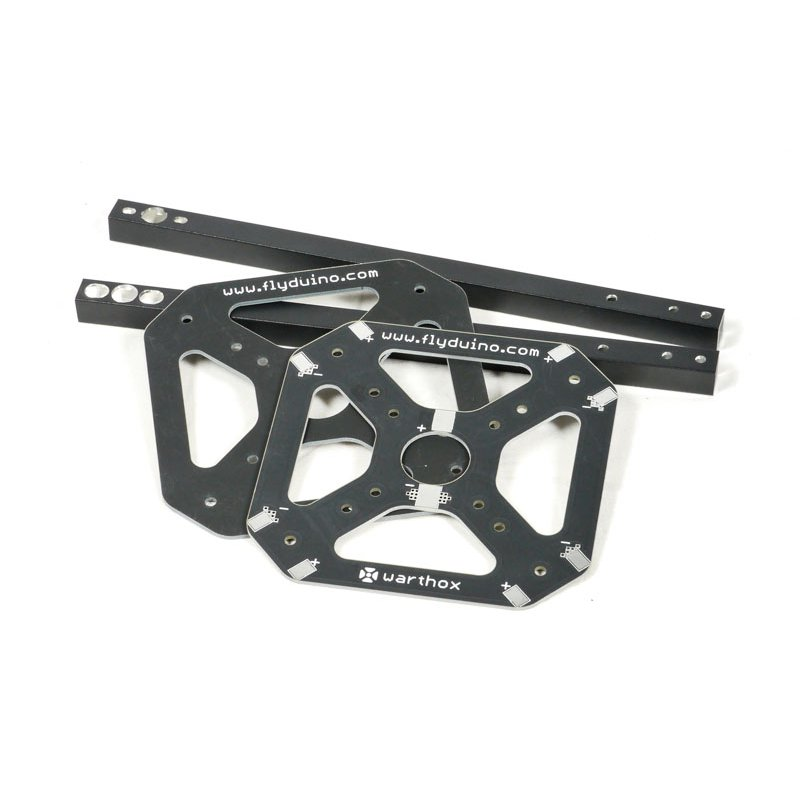
\includegraphics[scale=0.4]{Bilder/Quadrokopter-Rahmen.jpg}

\textbf{Preis:} 34,90 Euro

\subsection*{LiPo-Akku}
Ja nach Leistung unterschiedliche Größen wählbar. Für einen Nanoquad reichen 2S LiPo-Akkus mit 7,4V. Ansonsten werden in der Regel 3S LiPos, also Akkus mit 11,1V benötigt.

\subsubsection*{3S - 11,1V 2200mAh 20C}
\textbf{Preis:} 15,99 Euro

\subsubsection*{3S - 11,1V 2200mAh 30C}
\textbf{Preis:} 20,79 Euro

\subsubsection*{3S - 11,1V 3200mAh 30C}
\textbf{Preis:} 50,99 Euro

\subsubsection*{2S - 7,4V 1800mAh 30C}
\textbf{Preis:} 11,99 Euro

\subsection*{Kabel, Schrauben und Befestigungsmaterial}
Schrauben sind bei einzelnen Komponenten dabei. Bei Frame-Sets ist Befestigungsmaterial vorhanden. Bedacht werden sollte die Sicherung von Akku, Empfänger und Sensoren auf dem Rahmen. Möglichkeiten bieten hierzu:
\begin{itemize}
	\item Klettband
	\item klebbare Klettverschlüsse
	\item Kabelbinder
	\item Montagekleber
\end{itemize} 

\section*{Zusammenstellung verschiedener Konfigurationen}

\subsection*{Nanoquad}

\begin{tabular}{|c|c|c|c|}\hline
Komponente & Stück & Preis à Stück & Gesamtpreis\\\hline\hline
Rahmen & 1 & 34,99 & 34,99\\
Motor & 4 & 29,90 & 119,60\\
ESC & 4 & 12,49 & 49,96\\
FC & 1 & 38,90 & 38,90\\
Akku & 1 & 11,99 & 11,99\\
Propeller & 8 & 6,50 & 6,50\\\hline\hline
Summe: & & & 261,94 \\\hline\hline
\end{tabular}

\subsection*{Quadrocopter 20cm}

\begin{tabular}{|c|c|c|c|}\hline
Komponente & Stück & Preis à Stück & Gesamtpreis\\\hline\hline
Rahmen & 1 & 34,90 & 34,90\\
Motor & 4 & 14,95 & 59,80\\
ESC & 4 & 16,99 & 67,96\\
FC & 1 & 38,90 & 38,90\\
Akku & 1 & 11,99 & 15,99\\
Propeller & 8 & 4,20 & 4,20\\\hline\hline
Summe: & & & 221,75 \\\hline\hline
\end{tabular}

\end{document}
